\chapter{Sampling} \label{ch:sampling}

Statistics is very widely used in science, engineering and social science. From a broad view, any attempt trying to estimate an unknown value (for example, a parameter of a system, a property of the population) using its direct or indirect measurements (for example, outputs of the system, surveys conducted on randomly selected samples from the population) can be counted as an application of statistics.

Due to the measurement error, limitation of sample size, etc., we might not be able to get the accurate value of the unknown. Unavoidably, there is error between the estimates and the true value of the parameter. Statistics studies the methodologies to find the most probable estimate of the parameter by efficiently using the measurements and samples. It also quantitatively calculate the confidence level to the conclusions it draws.

Statistics starts from obtaining the measurements and samples, and using them to model the unknown parameter or population. Different sampling and modeling methods are introduced in this chapter. 

\section{Problem Formulation} \label{sec:statisticsproblemformulation}

Consider the following two problems.
\begin{enumerate}
	\item There is an unknown parameter in the system. The parameter can be measured either directly or indirectly, subject to measurement noise. The problem is to estimate the most probable value or range of the parameter.
	\item There is the population, and it is impossible to interview each element to get an aggregated feature of the population. However, it is possible to survey a small part of the population. The problem is to select samples from the population, conduct the survey, and using the survey results to estimate the interested aggregated feature or a probable range for that feature.
\end{enumerate}
These two problems seem to differ largely, but they are closely related in the mathematical insights, and can be formulated as the same (or very similar) problem. 

Let ``measurements'' and ``samples'' be used interchangeably. Denote the samples as $x_i$, $i=1,\ldots,m$, where $m$ is the total number of samples. Denote the parameter to be estimated by $\theta$. In both problems, the objective is to obtain an estimation of $\theta$, $\hat{\theta}$, using the samples $x_i$. 

\section{Sampling Methods}

Sampling methods can be a concern of Problem 2 introduced earlier in Section \ref{sec:statisticsproblemformulation}. 
When selecting samples from the population, it is critical to ensure that the selection is done randomly, and all elements in the population have a equal probability to be selected. 

Depending on whether an element can be selected multiple times, we have
\begin{itemize}
  \item Sampling with replacement: a member can be chosen more than once.
  \item Sampling without replacement: a member can be chosen no more than once.
\end{itemize}
Sometimes it is interesting to compare the differences of the two methods, especially when the population is finite. An obvious difference is that by using sampling with replacement all the samples can be considered as ``independent'': the previously selected samples would not affect the aggregated feature of the future samples. From this point of view, using sampling with replacement is equivalent of sampling from infinite population by thinking that the population is duplicated infinite times and each sample is done in an independent duplication.

While by using sampling without replacement, previous samples may change the distributions in the elements in the population, thus making the samples relevant. 

When the population size is much larger than the sample size, the choice of the two sampling methods may not make any visible difference in the conclusion.

For further demonstration of the differences between sampling with and without replacement, consider the following example. A set of $N$ random variables are generated from a Gaussian distribution as the population. Sample the population $M$ times using sampling with/without replacement. Calculate the sampled mean and compare it with the mean of the entire population.

In the first example, let $N=100$ and $M=500$. Figures \ref{ch:sampling:fig:sample-wr-n100} and \ref{ch:sampling:fig:sample-nwr-n100} gives the cumulative mean and variance of sampling with and without replacement, respectively. The mean and variance are given by red and blue curves, respectively. The statistics obtained from the cumulative samples and from the population are given by the solid and dashed curves, respectively. Notice that in Fig. \ref{ch:sampling:fig:sample-nwr-n100}, after number of samples exceeding $100$, the entire population has been sampled, and thus the sampling stops. This explains why its mean and variance stop fluctuating and converge to the population mean and variance respectively.

\begin{figure}
	\centering
	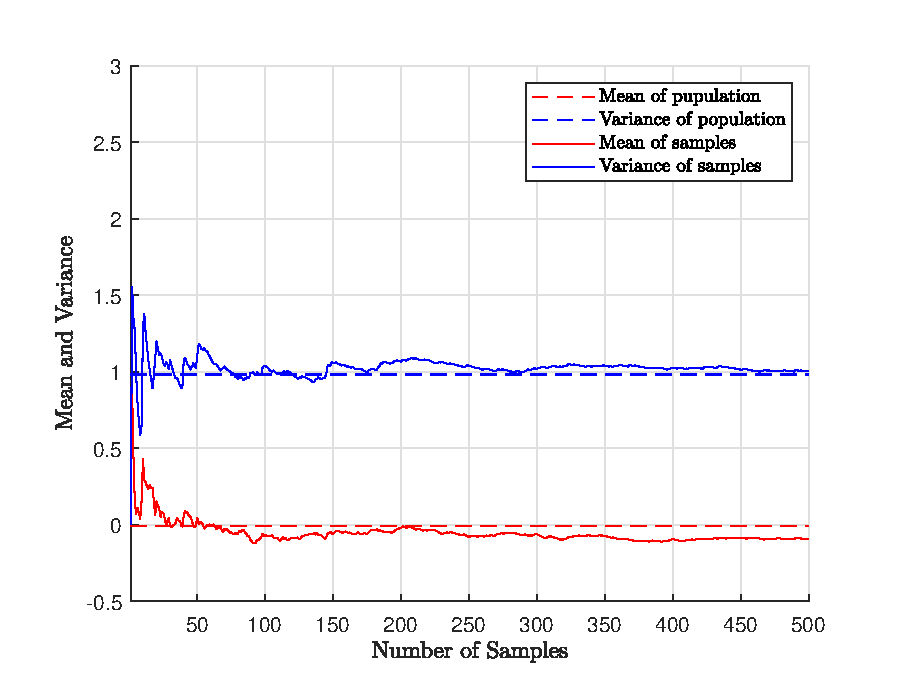
\includegraphics[width=250pt]{chapters/ch-sampling/figures/sample-wr-n100.eps}
	\caption{Sample with replacement, population size $N=100$, sample size $0< M\leq500$.} \label{ch:sampling:fig:sample-wr-n100}
\end{figure}

\begin{figure}
	\centering
	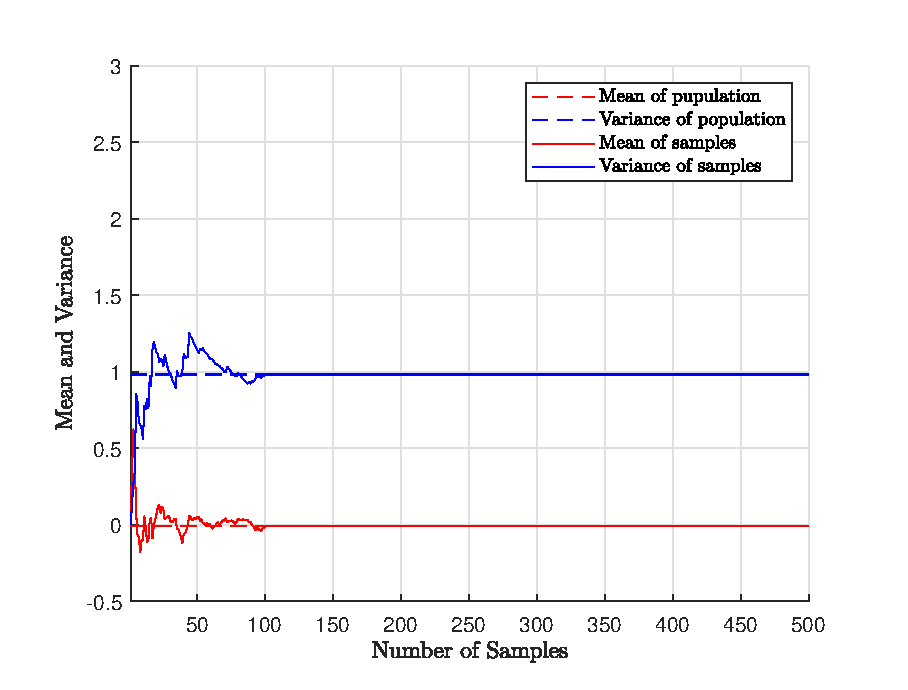
\includegraphics[width=250pt]{chapters/ch-sampling/figures/sample-nwr-n100.eps}
	\caption{Sample without replacement, population size $N=100$, sample size $0< M\leq500$.} \label{ch:sampling:fig:sample-nwr-n100}
\end{figure}

In practice, however, the population size is often orders of magnitudes larger than the number of samples. In the second example, let $N=10000$ and $M=500$. The corresponding figures are given in Figs. \ref{ch:sampling:fig:sample-wr-n10000} and \ref{ch:sampling:fig:sample-nwr-n10000}. There is no obvious differences of the two figures.

\begin{figure}
	\centering
	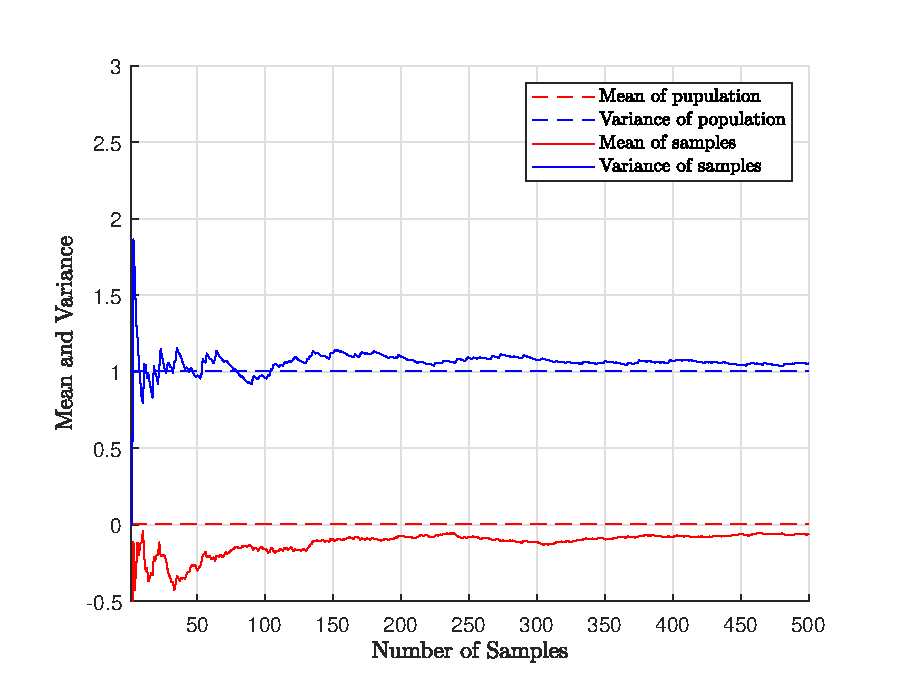
\includegraphics[width=250pt]{chapters/ch-sampling/figures/sample-wr-n10000.eps}
	\caption{Sample with replacement, population size $N=10000$, sample size $0< M\leq500$.} \label{ch:sampling:fig:sample-wr-n10000}
\end{figure}

\begin{figure}
	\centering
	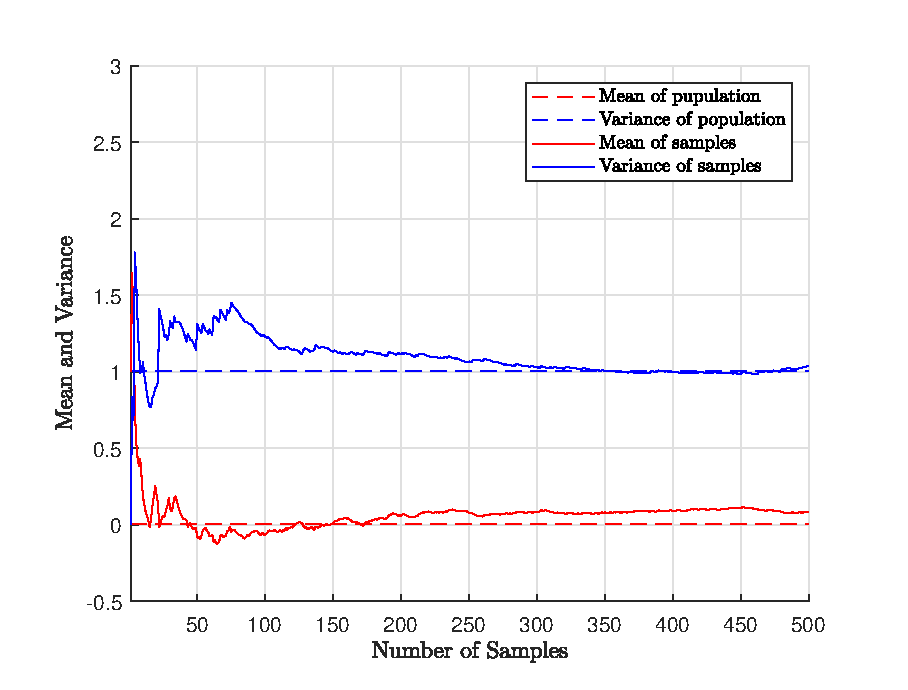
\includegraphics[width=250pt]{chapters/ch-sampling/figures/sample-nwr-n10000.eps}
	\caption{Sample without replacement,population size $N=10000$, sample size $0< M\leq500$.} \label{ch:sampling:fig:sample-nwr-n10000}
\end{figure}

\section{Models of Population}

The features of the population is often unknown, or at least not known precisely. It is common to make some preliminary assumptions to the distribution of the population using past experience.

For example, let $X$ be a feature of the population. It could be, for example, the heights of all teenagers in a city. We can make an assumption that $X$ follows Gaussian distribution with mean $\mu$ and standard deviation $\sigma$, and each element in the population, $X_i$, can be taken as a random variable generated from $f(x)$.

The preliminary assumptions of the population can be helpful in using the samples to model the population more efficiently. Of course, if the samples deny the assumption in the hypothesis test, the assumptions can be rejected and new models can be proposed.
